\chapter{Introduction}
This chapter provides an overview of the role of phosphates in biological systems, the enzymes involved in phosphate hydrolysis, and a detailed explanation of the reaction mechanisms associated with these processes--topics that have puzzled researchers for a long time. The discussion begins with the fundamental importance of phosphates in life, particularly in energy transfer and storage. This is followed by a brief overview of the enzymes that catalyse phosphate hydrolysis and their implications for cellular function. Finally, the chapter explores the reaction mechanisms of phosphate hydrolysis, highlighting key studies and findings in this area.

\section{Role of phosphates in biological systems}
Phosphates are among the fundamental building blocks that play a central role in life on Earth. They form the basis for both the storage and transfer of genetic information, as well as the flow of metabolic energy within biological systems. The ubiquitous nature of phosphate esters and anhydrides - such as those found in \ac{dna}, \ac{rna}, \ac{atp}, and \ac{polyp} - highlights their fundamental importance \citep{westheimerWhyNatureChose1987}. Some of the phosphates found in biological systems and their respective functions are summarised in Table~\ref{tab:role_of_phosphates}.

A key characteristic enabling these roles is the ability of phosphoric acid to link molecular units while retaining an ionisable group. This inherent negative charge at physiological pH serves a dual purpose: it helps to retain these molecules within cellular boundaries defined by lipid membranes, and more importantly, it confers kinetic stability upon phosphate esters and anhydrides by electrostatically repelling nucleophilic attack, particularly from water \citep{westheimerWhyNatureChose1987}. For instance, the half-time for hydrolysis at 25\textdegree{C} for a phosphomonoester monoanion (P-O) is about 90 years; however, for a phosphodiester anion (P-O), this number increases dramatically to approximately 16 million years \citep{wolfendenDegreesDifficultyWaterConsuming2006}. This stability is crucial for maintaining the integrity of genetic material but can be readily overcome by enzymatic catalysis when there is a metabolic demand.

Phosphates are involved in numerous processes in living systems, such as cell signalling and sensation, regulation of metabolism, blood coagulation, and bone formation \citep{mullerInorganicPolyphosphatesStorage2019, nebesnayaInorganicPolyphosphateRegulates2024}. Their role is perhaps most evident in cellular energetics, where \ac{atp} functions as the universal energy currency. The energy derived from nutrients such as glucose is captured and stored within the high-energy phosphoanhydride bonds linking the phosphate groups of \ac{atp}. This energy is released upon hydrolysis of the terminal phosphoanhydride bond (P-O bond between $\beta$ and $\gamma$ in Figure~\ref{fig:atp}), typically yielding \ac{adp} and \ac{Pi}. The cleavage of this bond provides the thermodynamic driving force for the majority of cellular processes, including biosynthesis, active transport, and mechanical work such as muscle contraction. The standard free energy change for ATP hydrolysis is substantial ($\Delta G^{0}=-30.5$ kJ mol$^{-1}$), and under cellular conditions, the actual free energy release is often considerably greater. Specifically, the experimentally obtained $\Delta G$ values are approximately $-59$ to $-53.5$ kJ mol$^{-1}$ in the liver and about $-61.7$ to $-59.5$ kJ mol$^{-1}$ in the heart \citep{mullerInorganicPolyphosphatesStorage2019}.

\begin{table}[b!]
    \centering
    \begin{tabular}{cc}
    \toprule
    \textbf{Phosphate} & \textbf{Biological role} \\ 
    \midrule
    DNA/RNA & Genetic material \\
    ADP/ATP & Intracellular energy transfer \\
    cAMP & Cellular signalling \\
    Polyphosphate & Energy storage, Cellular signalling \\
    Creatine phosphate & Intracellular energy transfer \\
    Phosphoenolpyruvate & Metabolism \\
    Pyridoxal phosphate & Coenzyme \\
    Nicotine adenine dinucleotide & Calcium signalling \\
    Fructose 1,6-diphosphate & Metabolism \\
    Glucose-6-phosphate & Metabolism \\
    Isopentenyl pyrophosphate & Metabolism \\
    Ribose-6-phosphate & Metabolism \\
    Glycerol 3-phosphate & Metabolism \\
    Dihydroxyacetone phosphate & Calvin cycle, metabolism \\
    Inositol phosphates & Cellular signalling \\
    \bottomrule
    \end{tabular}
    \caption{Examples of biologically relevant phosphates and their roles. Reproduced and adapted from~\citep{kamerlinWhyNatureReally2013}.}
    \label{tab:role_of_phosphates}
\end{table}

Beyond \ac{atp}, \ac{polyp} - a linear polymer of orthophosphate residues linked by similar high-energy phosphoanhydride bonds - represents another significant phosphate-based energy storage found across all domains of life, including mammalian cells. However, in mammalian cells, the concentration of \ac{polyp} is significantly lower compared to that in microorganisms. While its roles in mammals are still being fully elucidated, \ac{polyp} metabolism is intrinsically linked to the cellular energy status. Mitochondrial \ac{polyp} levels fluctuate with respiratory activity and appear to depend on F\textsubscript{0}F\textsubscript{1}-ATP synthase function, suggesting a role in mitochondrial bioenergetics, potentially acting as an energy reservoir \citep{pavlovInorganicPolyphosphateEnergy2010}.

The efficient transfer of energy stored in phosphate bonds from sites of production (e.g., mitochondria) to sites of utilisation (e.g., ATPases involved in muscle contraction or ion transport) is crucial. Simple diffusion of \ac{atp} is often insufficient due to the complexity of intracellular architecture and the potential for large concentration gradients to arise, which would be thermodynamically inefficient. Instead, cells employ phosphotransfer networks, utilising enzymes such as creatine kinase and adenylate kinase, which catalyse phosphoryl exchange reactions. These networks act as 'phosphoryl wires', facilitating the efficient conduction of high-energy phosphoryl groups and energetic signals throughout the cell with minimal energy dissipation or accumulation of inhibitory products such as \ac{adp}. The existence of these networks underscores the dynamic and highly organised nature of cellular energy management, where phosphates - mainly in the form of \ac{atp} - serve as the key energy carriers \citep{dzejaPhosphotransferNetworksCellular2003}.

The synthesis of \ac{atp} occurs primarily through oxidative phosphorylation in mitochondria, a process tightly coupled to the electron transport chain, which establishes a proton-motive force ($\Delta p$) across the inner mitochondrial membrane. This electrochemical potential energy is used by the molecular machine ATP synthase. Interestingly, the principal energy input required by ATP synthase is not for the chemical formation of the phosphoanhydride bond itself, but rather for the conformational changes necessary to release the newly synthesised, tightly bound \ac{atp} molecule from the enzyme's catalytic site. This 'binding change mechanism' involves the cooperative, sequential action of the enzyme's multiple catalytic sites, driven by proton flow. The hydrolysis of \ac{atp} to \ac{adp} and \ac{Pi} is catalysed by a variety of enzymes, including ATPases and possibly F\textsubscript{1}-ATPase, which are frequently coupled to other cellular processes \citep{boyerEnergyLifeATP1998}.

In summary, the unique chemical properties of phosphates - their ability to form stable esters and energy-rich anhydrides, along with their negative charge - combined with the evolution of sophisticated enzymatic machinery for their synthesis, transfer, and hydrolysis, have secured their vital role in virtually all life processes.



\section{Enzymes involved in phosphate hydrolysis}
The hydrolysis of high-energy phosphoanhydride bonds, particularly the terminal bond in \ac{atp}, is a cornerstone of cellular bioenergetics. While numerous enzymes utilise \ac{atp} hydrolysis, the F\textsubscript{0}F\textsubscript{1}-ATP synthase complex, primarily known for synthesising \ac{atp}, also shows potential \ac{atp} hydrolytic activity, particularly through its F\textsubscript{1} component (F\textsubscript{1}-ATPase). This enzyme complex, therefore, plays a dual role in managing the cell's primary energy currency \citep{bonoraATPSynthesisStorage2012, boyerEnergyLifeATP1998, walkerATPSynthaseUnderstood2013}. Furthermore, recent evidence suggests that this complex may also participate in the metabolism, including the hydrolysis, of \ac{polyp} in mammalian cells \citep{baevInorganicPolyphosphateF0F1ATP2022, baevInorganicPolyphosphateProduced2020}.

The F\textsubscript{0}F\textsubscript{1}-ATP synthase is a molecular motor embedded in the mitochondrial membrane. It consists of two major domains: the F\textsubscript{1} domain, which carries the catalytic sites, and the F\textsubscript{0} domain, which is embedded within the membrane. These domains are connected by a central rotor stalk and a peripheral stator stalk \citep{walkerATPSynthesisRotary1998, walkerATPSynthaseUnderstood2013, wattBioenergeticCostMaking2010}. The activity of this enzyme is coupled with the electron-transport chain, as illustrated in Figure~\ref{fig:atp_synthase}.

\begin{figure}[t!]
    \centering
    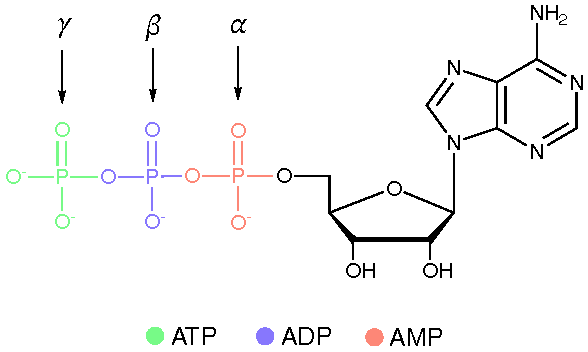
\includegraphics[width=0.6\textwidth]{Figures/1_Introduction/intro_atp.pdf}
    \caption{Chemical structures of the AMP, ADP, and ATP molecules with the phosphates marked as $\alpha$, $\beta$, and $\gamma$, respectively.}
    \label{fig:atp}
\end{figure}

The F\textsubscript{1} domain ($\alpha_3\beta_3\gamma\delta\epsilon$ stoichiometry) extends into the mitochondrial matrix. It has a globular shape as can be seen in Figure~\ref{fig:atp_synthase}. The catalytic sites for \ac{atp} synthesis and hydrolysis are located on the three $\beta$ subunits, which interact with the $\alpha$ subunits. When functioning in reverse, the F\textsubscript{1} domain acts as an F\textsubscript{1}-ATPase, hydrolysing \ac{atp}. This hydrolysis drives the counterclockwise rotation (as viewed from the membrane) of the central stalk, composed of the $\gamma$, $\delta$, and $\epsilon$ subunits \citep{walkerATPSynthesisRotary1998, walkerATPSynthaseUnderstood2013, boyerEnergyLifeATP1998}. If coupled to the F\textsubscript{0} domain, this rotation actively pumps protons from the matrix, thereby generating or maintaining the proton-motive force ($\Delta p$). This reverse function is especially important under conditions of low $\Delta p$, where it helps prevent its complete dissipation at the expense of cellular \ac{atp} and possibly \ac{polyp} \citep{bonoraATPSynthesisStorage2012, walkerATPSynthaseUnderstood2013, baevInorganicPolyphosphateProduced2020}.

The mechanism of \ac{atp} hydrolysis (cleavage of the P-O bond between $\beta$ and $\gamma$ in Figure~\ref{fig:atp}) follows the principles of the binding change mechanism \citep{walkerATPSynthaseUnderstood2013}. The rotation of the asymmetric $\gamma$ subunit induces sequential conformational changes in the three $\beta$ subunits, cycling them through states analogous to those in synthesis: an 'open' state that binds \ac{atp}, a 'tight' state that facilitates hydrolysis, and a subsequent 'open' state that releases \ac{adp} and \ac{Pi} \citep{walkerATPSynthesisRotary1998, boyerEnergyLifeATP1998}. The hydrolysis of each \ac{atp} molecule is associated with a 120\textdegree{} rotation of the central stalk, which occurs in substeps \citep{walkerATPSynthaseUnderstood2013}.

While the metabolism of inorganic \ac{polyp} is well-characterised in microorganisms via specific kinases (PPK) and phosphatases (PPX), the enzymes responsible for its turnover in mammalian cells remain largely unknown. Recent studies using immunocaptured F\textsubscript{0}F\textsubscript{1}-ATPase have demonstrated that the enzyme complex can hydrolyse \ac{polyp}. This \ac{polyp} hydrolysis appears to drive the enzyme's proton-pumping activity, akin to \ac{atp} hydrolysis, and is sensitive to oligomycin, a specific F\textsubscript{0}F\textsubscript{1}-ATP synthase inhibitor. Medium- and long-chain \ac{polyp} molecules, made of 60 and 130 orthophosphate units, respectively, seem to be effective substrates for this hydrolytic activity. Docking simulations support the feasibility of \ac{polyp} binding to the nucleotide-binding sites within the F\textsubscript{1} domain. This suggests that \ac{polyp} could serve as an alternative energy source for the F\textsubscript{0}F\textsubscript{1} complex, potentially helping to maintain mitochondrial membrane potential when \ac{atp} levels are compromised \citep{baevInorganicPolyphosphateProduced2020, baevInorganicPolyphosphateF0F1ATP2022}.

\begin{figure}[t!]
    \centering
    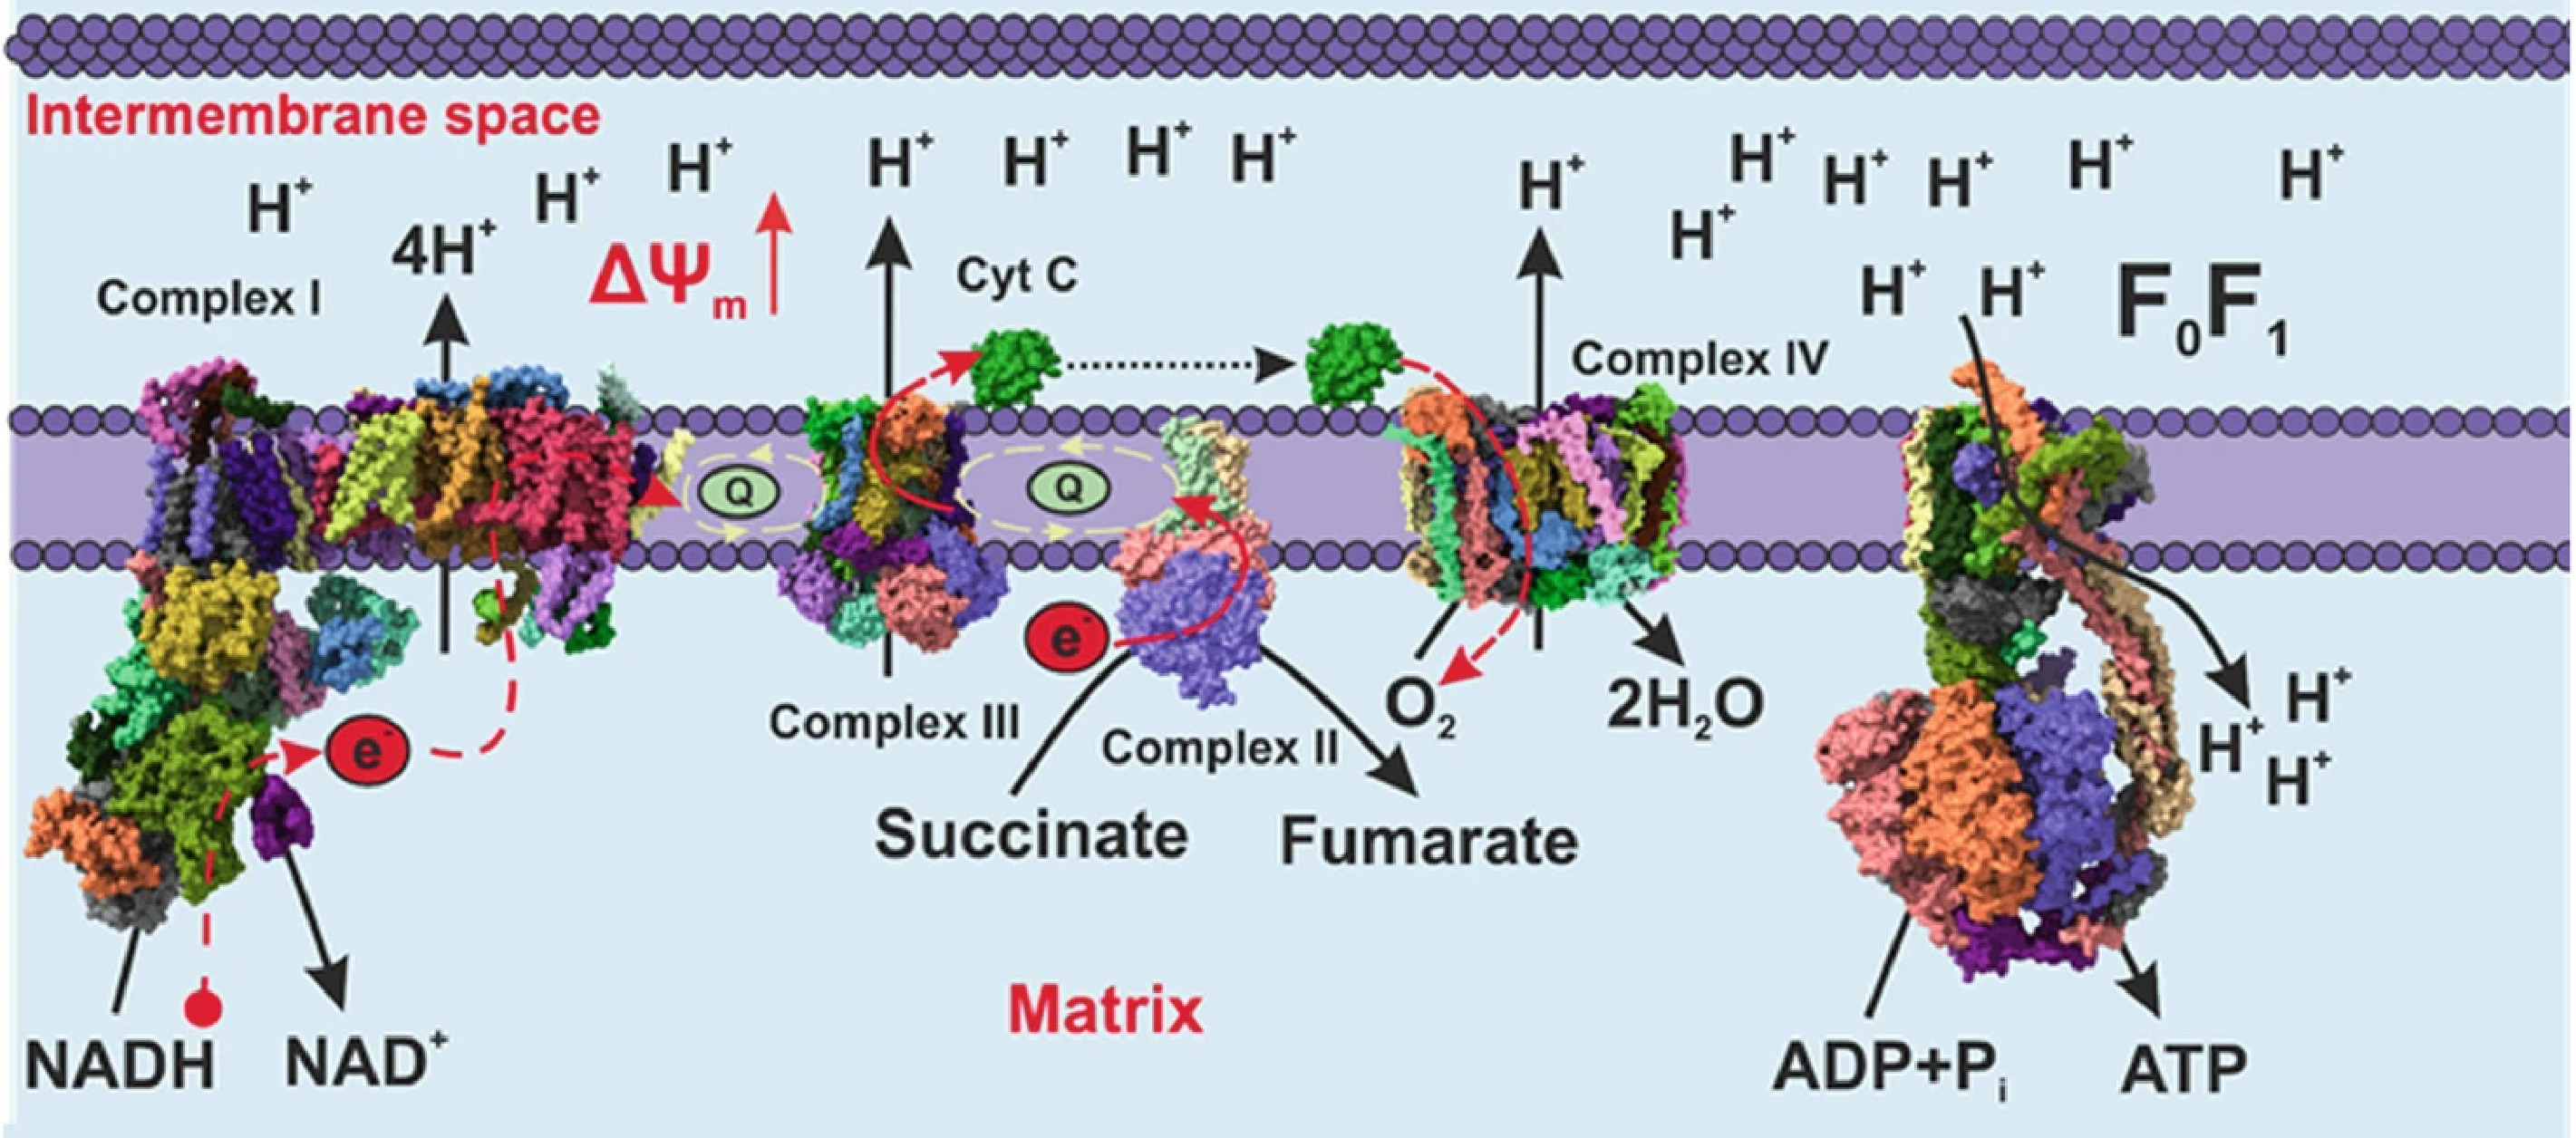
\includegraphics[width=0.95\textwidth]{Figures/1_Introduction/intro_atp_synthase.pdf}
    \caption{Electron transport chain coupled with oxidative phosphorylation in mitochondria. This figure was taken from \citep{baevInorganicPolyphosphateF0F1ATP2022}.}
    \label{fig:atp_synthase}
\end{figure}

There is growing confidence that the F\textsubscript{1}-ATPase could act not only as an \ac{atp} hydrolase but also potentially as a \ac{polyp} hydrolase. However, other enzymes contribute to phosphate metabolism as well. In the context of \ac{polyp}, mammalian enzymes such as alkaline phosphatase (ALP) have demonstrated exopolyphosphatase activity, capable of degrading \ac{polyp} chains of various lengths \citep{baevInorganicPolyphosphateF0F1ATP2022}.

The world of enzymes - and phosphate hydrolysis by F\textsubscript{1}-ATPase in particular - is both fascinating and complex. The F\textsubscript{1}-ATPase is a molecular machine capable of hydrolysing \ac{atp} and \ac{polyp}, yet the precise mechanism of hydrolysis remains not well understood. In order to address this gap, it is necessary to investigate the fundamental reaction mechanisms of phosphate hydrolysis, beginning with the simplest phosphate esters in less complex environments such as bulk water.



\section{Reaction mechanism: phosphate monoesters}
Computational and experimental studies have provided significant insights into the mechanisms of phosphate hydrolysis reactions. Various systems and methodologies have been employed to explore the details of these fundamental biological processes. The debate often centres on whether the reaction proceeds via an associative mechanism (bond formation precedes bond breaking) or a dissociative mechanism (bond breaking precedes bond formation), and the nature of the proton transfer.



\subsection{Phosphates} \label{subsec:phosphates}
Starting from the simplest possible system, it has been shown that the hydrolysis of \ac{memp} in water can proceed via either associative or concerted mechanisms \citep{kamerlinWhyNatureReally2013, kamerlinAssociativeDissociativeMechanisms2008, klahnMechanismHydrolysisPhosphate2006, duarteResolvingApparentConflicts2015}. A schematic representation of these mechanisms is presented in Figure~\ref{fig:mfj_plot}, which illustrates the More O'Ferrall-Jencks (MFJ) diagram. The MFJ plot is a useful two-dimensional graphical representation of multidimensional free energy surfaces.

The associative mechanism may proceed in two ways: stepwise (A\textsubscript{N} + D\textsubscript{N}, where A\textsubscript{N} stands for nucleophilic addition and D\textsubscript{N} for nucleophilic departure) or concerted (A\textsubscript{N}D\textsubscript{N}). The stepwise mechanism involves two transition states and an intermediate. In contrast, the concerted mechanism proceeds through a single transition state without the formation of intermediates \citep{duarteResolvingApparentConflicts2015}.

\begin{figure}[t!]
    \centering
    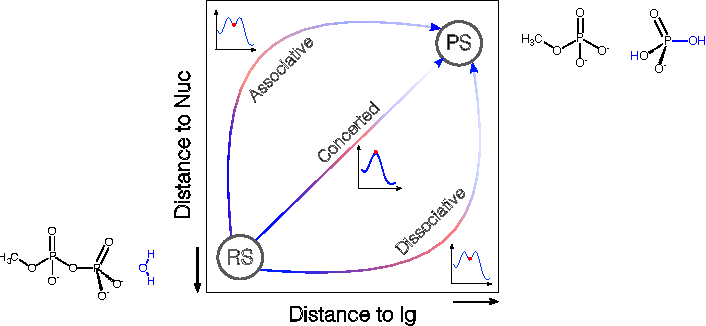
\includegraphics[width=0.95\textwidth]{Figures/1_Introduction/intro_mfj_plot.pdf}
    \caption{More O'Ferrall-Jencks (MFJ) plot of the possible reaction mechanisms for phosphate hydrolysis. The plot shows the free energy as a function of two reaction coordinates: the distance between phosphorus and the nucleophile (Nuc), and the distance between the leaving group (lg) and the phosphorus atom. RS stands for reactant state, PS for product state.}
    \label{fig:mfj_plot}
\end{figure}

In the case of the associative/stepwise mechanism (A\textsubscript{N} + D\textsubscript{N}, Figure~\ref{fig:reaction-mechanism}), the \ac{nuc} approaches the phosphorus atom while the \ac{lg} is still attached. Upon the nucleophile's approach, a concerted \ac{pt} occurs to one of the non-bridging oxygens. The reaction proceeds through a compact pentacoordinated transition state with a trigonal bipyramidal geometry, followed by a compact intermediate and the elimination of the leaving group in a subsequent transition state.

Regarding the associative/concerted mechanism (A\textsubscript{N}D\textsubscript{N}), it proceeds in a manner quite similar to the first step of the associative/stepwise pathway. The reaction also involves a compact transition state in which bond formation and bond cleavage occur simultaneously.

It has been shown that the protonation state of methyl phosphate lowers the overall barrier height of the rate-limiting step; however, it does not alter the reaction mechanism \citep{hassanEffectProtonationMechanism2017}. For the \ac{mehmp}, the calculated barrier height $\Delta G^{\ddagger}_{\text{calc}}$ is approximately 6-7 kcal/mol lower than that of the \ac{memp}. A similar effect was observed when OH\textsuperscript{-} acted as a nucleophile instead of a water molecule \citep{klahnMechanismHydrolysisPhosphate2006} (40 vs 47 kcal/mol, respectively). The latter fact arises a question about the proton-transfer in this reaction, for instance, whether it could happen in a concerted or a stepwise manner, in which the PT happens in the pre-equillibration phase.

For the associative mechanism, calculated barrier heights $\Delta G^{\ddagger}_{\text{calc}}$ lie in the range of 33.7-47.2 kcal/mol, while experimental values obtained at 25 \textdegree{C} range between 30.6 and 44.3 kcal/mol, depending on the protonation state. Detailed information about the calculated and experimentally determined barrier heights can be found in Table~\ref{tab:summary_comp_exp_barriers}. Corresponding data on transition state structures and intermediates is summarised in Table~\ref{tab:summary_ts_structures}.

\begin{figure}[t!]
    \centering
    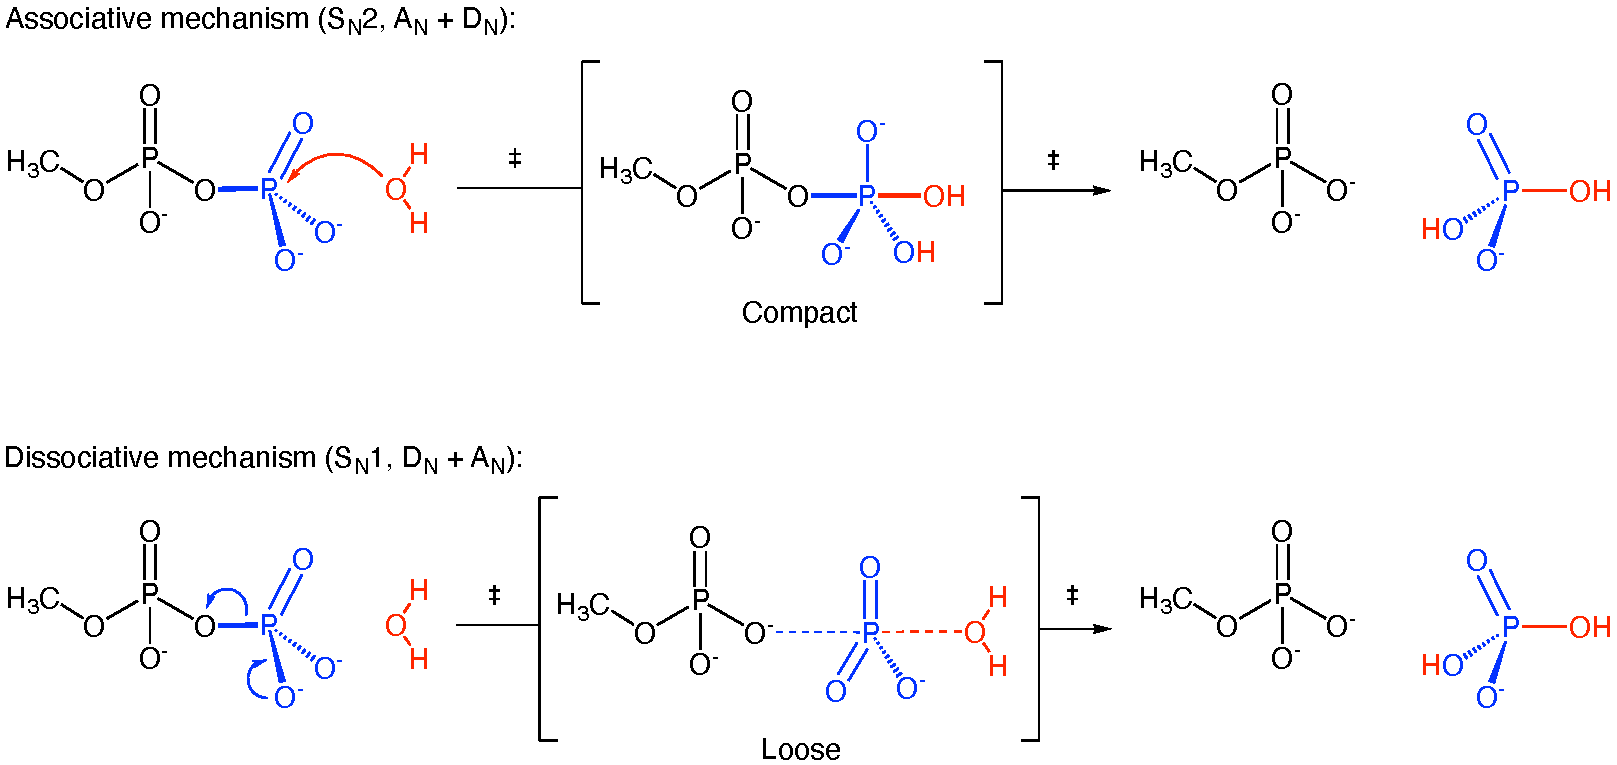
\includegraphics[width=0.95\textwidth]{Figures/1_Introduction/intro_reaction_mechanism.pdf}
    \caption{Associative and dissociative reaction mechanisms. For the transition states, only one of the two is shown. The nucleophile (Nuc) is shown in red, the leaving group (lg) in black, and the phosphoryl group in blue.}
    \label{fig:reaction-mechanism}
\end{figure}

The concerted mechanism (A\textsubscript{N}D\textsubscript{N}) is characterised by a single transition state \; where the nucleophile approaches the phosphorus atom while the leaving group remains attached. The reaction proceeds via a compact pentacoordinated transition state with a trigonal bipyramidal geometry, which is more expansive compared to that of the associative mechanism (Table~\ref{tab:summary_ts_structures}). In this transition state, the distance between the phosphorus atom and the nucleophile is approximately 2.06-2.75~\AA, while the distance between the leaving group and the phosphorus atom is around 2.61-2.75~\AA. The barrier heights for the concerted mechanism are 44.5 and 47 kcal/mol (Table~\ref{tab:summary_comp_exp_barriers}).

As can be observed, it is rather difficult to clearly distinguish between the associative and concerted mechanisms, and it appears that both may occur in bulk water. Even by looking at the activation entropies of both reaction pathways, it's clear that the corresponding values are similarly small: 0.7 and -1.6 kcal/mol for the associative and concerted mechanisms, respectively \citep{duarteResolvingApparentConflicts2015}.  Nevertheless, the dissociative mechanism is unlikely to take place, or at least it has not been observed.



\subsection{Diphosphates}
Moving on to more complex systems, the hydrolysis of pyrophosphates (diphosphates) (e.g. \ac{medp}), which are the main focus of this thesis, has also been thoroughly studied. It has been shown that the reaction mechanism can proceed through either associative or concerted pathways, just as in the case of methyl phosphate. In contrast, the associative mechanism has been demonstrated to be solely concerted. However, there is a twist to this story: the dissociative mechanism has also been observed, in both concerted and stepwise forms \citep{klahnMechanismHydrolysisPhosphate2006, kamerlinAssociativeDissociativeMechanisms2008, prasadAddressingOpenQuestions2013}. A schematic representation of the mechanisms can be found in Figures~\ref{fig:mfj_plot} and \ref{fig:reaction-mechanism}.

In the associative/concerted mechanism, the reaction undergoes the same steps as discussed in Subsection~\ref{subsec:phosphates}. The transition state has a similarly compact geometry: the distance between the phosphorus atom and the nucleophile is approximately 2.03--2.26~\AA, and the distance between the leaving group and the phosphorus atom is around 1.82--2.4~\AA, as shown in Table~\ref{tab:summary_ts_structures}. However, the calculated barrier heights are slightly lower in comparison to methyl phosphate, ranging from 34 to 38 kcal/mol (Table~\ref{tab:summary_comp_exp_barriers}).

\begin{table}[htbp]
    \centering
    \small
    \caption{Summary of computational and experimental studies on phosphate hydrolysis. In the case of calculated $\Delta G^\ddagger$, the rate-limiting step is given. \textsuperscript{1}The values were calculated using the transition state theory (TST).}
    \label{tab:summary_comp_exp_barriers}
    \resizebox{\textwidth}{!}{%
    \renewcommand{\arraystretch}{1.3}
    \begin{tabular}{@{}p{4.5cm} p{2.5cm} p{4.0cm} p{3.0cm} p{3.0cm} p{1.0cm}@{}}
    \toprule
    \textbf{System} & \textbf{Method} & \textbf{Level of theory} & \textbf{Mechanism} & \textbf{\boldmath$\Delta G^\ddagger$ (kcal/mol)} & \textbf{Ref.} \\ \midrule
    
    MeMP$^{2-}$ + H$_2$O & 
    DFT & B3LYP/6-311+G** and COSMO &
    Associative \newline Concerted & 
    47.2 \newline 44.5 & 
    \citep{kamerlinAssociativeDissociativeMechanisms2008} \\
    
    MeMP$^{2-}$ + H$_2$O & 
    DFT & B3LYP/6-311++G** and COSMO & 
    Associative & 
    47 & 
    \citep{klahnMechanismHydrolysisPhosphate2006} \\
    
    MeMP$^{2-}$ + 3 H$_2$O & 
    DFT & M06-2X/6-311+G** and SMD &
    Associative \newline Concerted & 
    $\approx$ 36 \newline $\approx$ 44 & 
    \citep{duarteResolvingApparentConflicts2015} \\
    
    MeMP$^{2-}$ + 4 H$_2$O & 
    DFT & M06-2X/6-311+G** &
    Associative & 
    $\approx$ 40.8$\pm$1.9 & 
    \citep{hassanEffectProtonationMechanism2017} \\
    
    MeHMP$^{-}$ + 4 H$_2$O & 
    DFT & M06-2X/6-311+G** &
    Associative & 
    $\approx$ 33.7$\pm$1.7 & 
    \citep{hassanEffectProtonationMechanism2017} \\
    
    MeDP$^{3-}$ + 2 H$_2$O & 
    DFT & B3LYP/6-311++G** and PCM & 
    Associative \newline Dissociative & 
    34.64 \newline 35.24 & 
    \citep{prasadAddressingOpenQuestions2013} \\
    
    MeDP$^{3-}$ + H$_2$O & 
    DFT & B3LYP/6-311+G** and COSMO & 
    Associative \newline Dissociative & 
    34.8 \newline 30.3 & 
    \citep{kamerlinAssociativeDissociativeMechanisms2008} \\
    
    MeDP$^{3-}$ + H$_2$O & 
    DFT & B3LYP/6-311++G** and COSMO & 
    Associative \newline Concerted & 
    38 \newline 34 & 
    \citep{klahnMechanismHydrolysisPhosphate2006} \\
    
    MeHDP$^{2-}$ + H$_2$O & 
    DFT & B3LYP/6-311++G** and COSMO & 
    Associative \newline Concerted & 
    34 \newline 31 & 
    \citep{klahnMechanismHydrolysisPhosphate2006} \\
    
    MeDP$^{3-}$ + Mg$^{2+}$ + 5 H$_2$O & 
    QM/MM, \newline FEP (EVB) & B3LYP/6-311++G** and MM & 
    Associative \newline Concerted \newline Dissociative & 
    35 \newline 34 \newline 35 & 
    \citep{klahnMechanismHydrolysisPhosphate2006} \\

    MeTP$^{4-}$ + Mg$^{2+}$ + 54 H$_2$O & 
    CPMD & PBE/PW with Troullier-Martins pseudopotentials & 
    Associative \newline Concerted \newline Dissociative & 
    39.1 \newline 35.1 \newline 36.6 & 
    \citep{akolaATPHydrolysisWater2003} \\
    
    MeTP$^{4-}$ + Mg$^{2+}$ + 113 H$_2$O & 
    BOMD, \newline metadynamics & BLYP/TZV2P with GTH pseudopotentials & 
    Associative \newline Concerted & 
    29 \newline 29-30 & 
    \citep{glavesMechanisticInsightsHydrolysis2012} \\

    ATP$^{4-}$ + Mg$^{2+}$ + 4163 H$_2$O + counterions & 
    QM/MM, NEB & B3LYP/6-311++G** and MM & 
    Concerted & 
    32.5 & 
    \citep{wangQMMMInvestigation2015} \\
    
    ATP$^{4-}$ + Mg$^{2+}$ + 1800 H$_2$O + counterions & 
    QM/MM, QM = CPMD & BLYP/PW with Troullier-Martins pseudopotentials and MM & 
    Associative \newline Dissociative & 
    36.2 \newline 33.4 & 
    \citep{harrisonQuantumClassicalDynamics2012} \\
    
    \midrule
    
    Methyl phosphate \newline dianion & 
    Exp. at 25\textdegree{C} & 
    -- & -- & 
    44.3 & 
    \citep{wolfendenDegreesDifficultyWaterConsuming2006} \\
    
    Methyl phosphate \newline monoanion & 
    Exp. at 25\textdegree{C} & 
    -- & -- & 
    30.6 & 
    \citep{wolfendenDegreesDifficultyWaterConsuming2006} \\
    
    Pyrophosphate trianion & 
    Exp. at 25\textdegree{C} & 
    -- & -- & 
    29.2 & 
    \citep{wolfendenDegreesDifficultyWaterConsuming2006} \\
    
    Pyrophosphate dianion & 
    Exp. at 25\textdegree{C} & 
    -- & -- & 
    27.7 & 
    \citep{wolfendenDegreesDifficultyWaterConsuming2006} \\
    
    ADP$^{2-}$ (or ATP$^{3-}$) & 
    Exp. at 25\textdegree{C} & 
    -- & -- & 
    27.5 & 
    \citep{wolfendenDegreesDifficultyWaterConsuming2006} \\
    
    ATPH$^{3-}$ (or ATP$^{4-}$) & 
    Exp. at 70\textdegree{C} & 
    pH=6.69-7.66 & -- & 
    24.34-24.78\textsuperscript{1} & 
    \citep{ramirezMagnesiumCalciumIon1980} \\
    
    dADPH$^{2-}$ (or dADP$^{3-}$) & 
    Exp. at 70\textdegree{C} & 
    pH=6.82 & -- & 
    24.25\textsuperscript{1} & 
    \citep{ramirezComparativeStudyHydrolysis1982a} \\
    
    dATPH$^{3-}$ (or dATP$^{4-}$) & 
    Exp. at 70\textdegree{C} & 
    pH=7.00  & -- & 
    24.50\textsuperscript{1} & 
    \citep{ramirezComparativeStudyHydrolysis1982a} \\
    
    MgATPH$^{-}$ (or MgATP$^{2-}$) & 
    Exp. at 70\textdegree{C} & 
    pH=6.59-7.63  & -- & 
    24.59-24.64\textsuperscript{1} & 
    \citep{ramirezMagnesiumCalciumIon1980} \\
    
    CaATPH$^{-}$ (or CaATP$^{2-}$) & 
    Exp. at 70\textdegree{C} & 
    pH=6.67-7.01 & -- & 
    25.71-25.72\textsuperscript{1} & 
    \citep{ramirezMagnesiumCalciumIon1980} \\
    
    \bottomrule
    \end{tabular}%
    }
\end{table}

The concerted pathway is characterised by the same general mechanism as discussed in Subsection~\ref{subsec:phosphates}. The transition state is more expansive than in the associative mechanism, with the distance between the phosphorus atom and the nucleophile being approximately 2.26--2.5~\AA, while the distance between the leaving group and the phosphorus atom is around 2.7~\AA\ (Table~\ref{tab:summary_ts_structures}). The barrier heights for the concerted mechanism are 31 and 34 kcal/mol (Table~\ref{tab:summary_comp_exp_barriers}), which is notably lower than in the case of methyl phosphate.

In general, it can be noted that the barrier height is strongly dependent on the $pK_a$ value of the leaving group. The lower the $pK_a$, the lower the $\Delta G^{\ddagger}$ ($pK_a$(CH\textsubscript{3}O\textsuperscript{-}) $= 15.5$ vs $pK_a$(CH\textsubscript{3}PO\textsubscript{4}\textsuperscript{2-}) $= 6.3$). Not only does a lower $pK_a$ reduce the barrier height, but it also favours the concerted and dissociative mechanisms \citep{klahnMechanismHydrolysisPhosphate2006}.

The dissociative mechanism can proceed via both concerted and stepwise routes. The dissociative/concerted pathway is quite similar to the general concerted mechanism. The main difference lies in the synchrony of the transition state: while the general concerted mechanism has a more synchronous transition state, the dissociative/concerted one features a greater distance between the phosphorus atom and the leaving group.

On the other hand, the dissociative/stepwise pathway (D\textsubscript{N} + A\textsubscript{N}) is characterised by the departure of the leaving group from the phosphorus atom before the nucleophile approaches. Thus, there is clearly no bond remaining between the phosphorus and the leaving group. Following the departure of the leaving group, a planar metaphosphate PO\textsubscript{3}\textsuperscript{-} is formed, as illustrated in Figure~\ref{fig:reaction-mechanism}. The transition state is more expansive compared to that of the associative mechanism, with the distance between the phosphorus atom and the nucleophile being 2.7~\AA, and the distance between the leaving group and the phosphorus atom being 3.4~\AA\ (Table~\ref{tab:summary_ts_structures}). Consequently, after TS\textsubscript{1}, the system reaches an intermediate step in which the nucleophile is positioned closer to the metaphosphate, followed by an attack and bond formation in TS\textsubscript{2}.

The barrier heights for the dissociative mechanism lie in the range of 30.3--35.24 kcal/mol (Table~\ref{tab:summary_comp_exp_barriers}), which is lower than those for any of the previously mentioned mechanisms. Comparing the calculated and experimentally obtained $\Delta G^{\ddagger}$ clearly indicates that the dissociative mechanism is more favourable than the associative and concerted ones. The $\Delta G^{\ddagger}_{\text{exp}}$ values for the pyrophosphate trianion and dianion are 29.2 and 27.7 kcal/mol, respectively. The influence of one-water (1W) or two-water (2W) mechanisms has also been explored \citep{prasadAddressingOpenQuestions2013}, but the overall barriers remain similar.

The dissociative mechanism is further favoured by the presence of metal ions, such as Mg\textsuperscript{2+}, as well as in cases where \ac{medp} is protonated, i.e. \ac{mehdp}. Interestingly, in the latter case, the proton always transfers to the leaving group en route to the product state \citep{klahnMechanismHydrolysisPhosphate2006}.

\begin{table}[htbp]
    \centering
    \small
    \caption{Summary of the distances between the phosphorus atom and the nucleophile as well as the leaving group in the transition states and intermediates. All distances are in \AA.}
    \label{tab:summary_ts_structures}
    \resizebox{\textwidth}{!}{%
    \renewcommand{\arraystretch}{1.2}
    \begin{tabular}{@{}p{2.0cm} p{2.0cm} 
                    >{\centering\arraybackslash}p{2.16cm} 
                    >{\centering\arraybackslash}p{2.16cm} 
                    >{\centering\arraybackslash}p{2.16cm} 
                    >{\centering\arraybackslash}p{2.16cm} 
                    >{\centering\arraybackslash}p{2.16cm} 
                    >{\centering\arraybackslash}p{2.16cm} 
                    p{1.0cm}@{}}
    \toprule
    \textbf{System} & \textbf{Mechanism} & 
    \multicolumn{2}{c}{\textbf{TS\textsubscript{1}}} & 
    \multicolumn{2}{c}{\textbf{Intermediate}} & 
    \multicolumn{2}{c}{\textbf{TS\textsubscript{2}}} & 
    \textbf{Ref.} \\
    \cmidrule(lr){3-4} \cmidrule(lr){5-6} \cmidrule(lr){7-8}
    & & \textbf{d(P-O\textsubscript{Nuc})} & \textbf{d(P-O\textsubscript{lg})} & 
            \textbf{d(P-O\textsubscript{Nuc})} & \textbf{d(P-O\textsubscript{lg})} & 
            \textbf{d(P-O\textsubscript{Nuc})} & \textbf{d(P-O\textsubscript{lg})} & \\ 
    \midrule

    MeMP$^{2-}$ & 
    Associative (A\textsubscript{N}D\textsubscript{N}) & 
    2.0 & 1.8 & 
    -- & -- & 
    -- & -- & 
    \citep{klahnMechanismHydrolysisPhosphate2006} \\

    & 
    Associative (A\textsubscript{N}D\textsubscript{N}) & 
    1.9 & 2.15 & 
    -- & -- & 
    -- & -- & 
    \citep{kamerlinAssociativeDissociativeMechanisms2008} \\

    & 
    Associative (A\textsubscript{N} + D\textsubscript{N}) & 
    2.16 & 1.71 & 
    1.84 & 1.78 & 
    1.71 & 2.24 & 
    \citep{duarteResolvingApparentConflicts2015} \\

    & 
    Associative (A\textsubscript{N} + D\textsubscript{N}) & 
    2.08 & 1.78 & 
    1.99 & 1.80 & 
    1.77 & 2.52 & 
    \citep{hassanEffectProtonationMechanism2017} \\

    & 
    Concerted (A\textsubscript{N}D\textsubscript{N}) & 
    2.75 & 2.75 & 
    -- & -- & 
    -- & -- & 
    \citep{kamerlinAssociativeDissociativeMechanisms2008} \\

    & 
    Concerted (A\textsubscript{N}D\textsubscript{N}) & 
    2.06 & 2.61 & 
    -- & -- & 
    -- & -- & 
    \citep{duarteResolvingApparentConflicts2015} \\

    MeHMP$^{-}$& 
    Associative (A\textsubscript{N} + D\textsubscript{N}) & 
    2.26 & 1.66 & 
    1.76 & 1.77 & 
    1.68 & 2.25 & 
    \citep{hassanEffectProtonationMechanism2017} \\

    \midrule

    MeDP$^{3-}$& 
    Associative (A\textsubscript{N}D\textsubscript{N}) & 
    2.2 & 2.0 & 
    -- & -- & 
    -- & -- & 
    \citep{kamerlinAssociativeDissociativeMechanisms2008} \\

    & 
    Associative (A\textsubscript{N}D\textsubscript{N}) & 
    2.03 & 1.88 & 
    -- & -- & 
    -- & -- & 
    \citep{klahnMechanismHydrolysisPhosphate2006} \\
    
    & 
    Associative (A\textsubscript{N}D\textsubscript{N}) & 
    2.2 & 2.0 & 
    -- & -- & 
    -- & -- & 
    \citep{prasadAddressingOpenQuestions2013} \\

    &
    Concerted (A\textsubscript{N}D\textsubscript{N}) & 
    2.5 & 2.7 & 
    -- & -- & 
    -- & -- & 
    \citep{klahnMechanismHydrolysisPhosphate2006} \\

    & 
    Dissociative (A\textsubscript{N}D\textsubscript{N}) & 
    2.8 & 3.25 & 
    -- & -- & 
    -- & -- & 
    \citep{kamerlinAssociativeDissociativeMechanisms2008} \\

    & 
    Dissociative (D\textsubscript{N} + A\textsubscript{N}) & 
    2.7 & 3.4 & 
    2.0 & 3.75 & 
    1.7 & 3.75 & 
    \citep{prasadAddressingOpenQuestions2013} \\

    MeDP$^{3-}$ \newline + Mg$^{2+}$ &
    Associative (A\textsubscript{N}D\textsubscript{N}) &
    2.1 & 2.4 & 
    -- & -- & 
    -- & -- & 
    \citep{klahnMechanismHydrolysisPhosphate2006} \\

    &
    Concerted (A\textsubscript{N}D\textsubscript{N}) &
    2.3 & 2.7 & 
    -- & -- & 
    -- & -- & 
    \citep{klahnMechanismHydrolysisPhosphate2006} \\

    &
    Dissociative (A\textsubscript{N}D\textsubscript{N}) &
    2.8 & 3.4 & 
    -- & -- & 
    -- & -- & 
    \citep{klahnMechanismHydrolysisPhosphate2006} \\

    MeHDP$^{2-}$& 
    Associative (A\textsubscript{N}D\textsubscript{N}) & 
    2.26 & 1.82 & 
    -- & -- & 
    -- & -- & 
    \citep{klahnMechanismHydrolysisPhosphate2006} \\

    &
    Concerted (A\textsubscript{N}D\textsubscript{N}) & 
    2.26 & 2.78 & 
    -- & -- & 
    -- & -- & 
    \citep{klahnMechanismHydrolysisPhosphate2006} \\
    
    \midrule

    MeTP$^{4-}$ \newline + Mg$^{2+}$&
    Associative (A\textsubscript{N}D\textsubscript{N}) & 
    1.9 & 2.0 & 
    -- & -- & 
    -- & -- & 
    \citep{akolaATPHydrolysisWater2003} \\

    & Associative (A\textsubscript{N} + D\textsubscript{N}) & 
    2.03 & 3.11 & 
    1.95 & 3.06 & 
    1.66 & 3.26 & 
    \citep{glavesMechanisticInsightsHydrolysis2012} \\

    &
    Concerted (A\textsubscript{N}D\textsubscript{N}) & 
    2.5 & 2.6 & 
    -- & -- & 
    -- & -- & 
    \citep{akolaATPHydrolysisWater2003} \\

    &
    Concerted (A\textsubscript{N}D\textsubscript{N}) & 
    2.28 & 2.69 & 
    -- & -- & 
    -- & -- & 
    \citep{glavesMechanisticInsightsHydrolysis2012} \\

    &
    Dissociative (A\textsubscript{N}D\textsubscript{N}) & 
    3.6 & 3.5 & 
    -- & -- & 
    -- & -- & 
    \citep{akolaATPHydrolysisWater2003} \\

    ATP$^{4-}$ \newline + Mg$^{2+}$ &
    Associative (A\textsubscript{N}D\textsubscript{N}) & 
    1.9 & 1.9 & 
    -- & -- & 
    -- & -- & 
    \citep{harrisonQuantumClassicalDynamics2012} \\
    
    &
    Concerted (A\textsubscript{N}D\textsubscript{N}) & 
    2.8 & 3.2 & 
    -- & -- & 
    -- & -- & 
    \citep{wangQMMMInvestigation2015} \\

    &
    Dissociative (A\textsubscript{N}D\textsubscript{N}) & 
    3.5 & 3.5 & 
    -- & -- & 
    -- & -- & 
    \citep{wangQMMMInvestigation2015} \\

    \bottomrule
    \end{tabular}%
    }
\end{table}

Even though computational studies suggest that Mg\textsuperscript{2+} promotes the dissociative mechanism, experimental data do not support this hypothesis \citep{ramirezMagnesiumCalciumIon1980}, since the $\Delta G^{\ddagger}_{\text{exp}}$ obtained at 70\textdegree{C} shows little to no difference, at least in the case of adenosine triphosphate (Table~\ref{tab:summary_comp_exp_barriers}).



\subsection{Triphosphates}
Last but not least, let us consider the hydrolysis of triphosphates. These systems more closely resemble the biological environment, particularly the processes associated with energy metabolism.

The hydrolysis of \ac{metp} and \ac{atp} has been studied using a range of computational methods. It has been shown that the reaction mechanisms share many similarities with those observed in mono- and diphosphates. Specifically, the mechanism may proceed via associative/concerted and associative/stepwise routes, as well as concerted and dissociative/concerted pathways (Table~\ref{tab:summary_ts_structures}). 

When comparing the calculated and experimentally obtained $\Delta G^{\ddagger}$ values, it is difficult to clearly distinguish between the aforementioned mechanisms. The calculated barrier heights span a range from 29 to 39.1 kcal/mol, whereas experimental data suggest that the barrier height for ATP should be around 27.5 kcal/mol, as shown in Table~\ref{tab:summary_comp_exp_barriers}. The more complex the system becomes, the more factors one must likely take into account.

In summary, computational investigations reveal a nuanced and peculiar picture of phosphate hydrolysis. The preferred mechanism (associative, concerted, or dissociative) and the proton transfer route (1W, 2W, etc.) depend significantly on specific factors such as the pKa of the leaving group, the protonation state, the presence of metal ions like Mg$^{2+}$, and the surrounding solvent environment. 



\section{Research goals}

To properly study the underlying free energy surface of the reaction mechanism, adequate sampling of the configurational space is crucial. To achieve this, various free energy techniques, such as metadynamics, can be employed - provided that the level of theory is sufficient to describe a system of realistic size while allowing results to be obtained within a reasonable timeframe. This is precisely the goal of the present project.

As a model system, methyl diphosphate hydrolysis in water has been chosen. Methyl diphosphate is a relatively simple phosphate ester that can represent more complex molecules like \ac{adp} and \ac{atp}. The main focus of this thesis is to investigate the reaction mechanism of \ac{medp} hydrolysis in water using well-tempered metadynamics, and to explore the influence of the protonation state and the solvent environment on the reaction mechanism. To run the metadynamics simulations, a neural network potential will be trained, thus allowing \textit{ab initio} molecular dynamics simulations to be performed at low computational cost.

Specifically, the following goals have been set for this thesis:
\begin{itemize}
    \item Compose a comprehensive dataset of molecular configurations covering all steps of the methyl diphosphate hydrolysis reaction mechanism.
    \item Train the NequIP neural network to fit a neural network potential that serves as an engine for the \textit{ab initio} molecular dynamics simulations.
    \item Assess the accuracy and performance of the neural network potential with respect to network complexity and the size of the training set.
    \item Perform extensive well-tempered metadynamics simulations to obtain the free energy surface of the methyl diphosphate hydrolysis reaction mechanism.
    \item Gain insights into the reaction mechanism, i.e. the kinetics and thermodynamics of the reaction, and compare the results with previously published data.
    \item Gain insights into the proton transfer mechanism.
\end{itemize}

Taking the above-mentioned goals into account, the present thesis follows the idea of Paul A. M. Dirac~\citep{diracQuantumMechanicsManyelectron1997}, who emphasised the need for approximate practical methods in quantum mechanics to explain complex atomic systems without excessive computational demands: 

\begin{displayquote}
    The underlying physical laws necessary for the mathematical theory of a large part of physics and the whole of chemistry are thus completely known, and the difficulty is only that the exact application of these laws leads to equations much too complicated to be soluble. \textit{It therefore becomes desirable that approximate practical methods of applying quantum mechanics should be developed, which can lead to an explanation of the main features of complex atomic systems without too much computation.}
\end{displayquote}

The use of neural network potentials in this thesis aims to achieve precisely that: to provide a practical and efficient approach to studying the reaction mechanism while maintaining a high level of accuracy.
